\documentclass[10pt]{beamer}
%\usepackage{ucltemplate}
\usepackage{pstricks,pst-node,pst-text,pst-3d,hyperref,color,epsfig,eurosym}
\usepackage[UKenglish]{babel}
\usefonttheme[onlymath]{serif}

\mode<presentation>
\usetheme{default} %Boadilla Singapore Warsaw
%\usetheme{Boadilla}
%\setbeamercovered{transparent} %
\setbeamertemplate{itemize item}{$\bullet$} %
\setbeamertemplate{itemize subitem}{--} %
\setbeamertemplate{navigation symbols}{}

\begin{document}

%\frame{%
%\frametitle{}%
%\begin{center}
%\rput(3.4,0.05){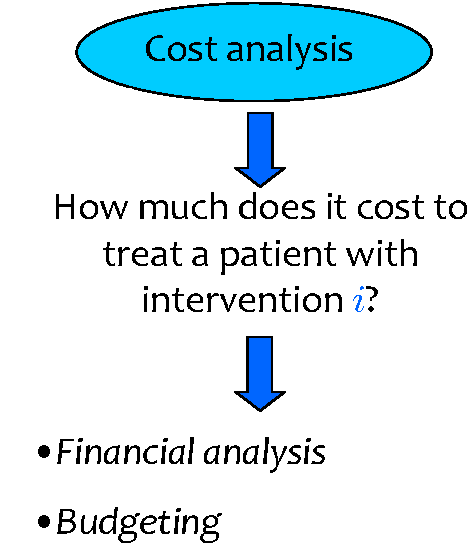
\includegraphics[width=3.8cm,angle=-90]{/home/gianluca/Dropbox/Unimib/MasterHE/he1}}
%\rput(-2.5,0){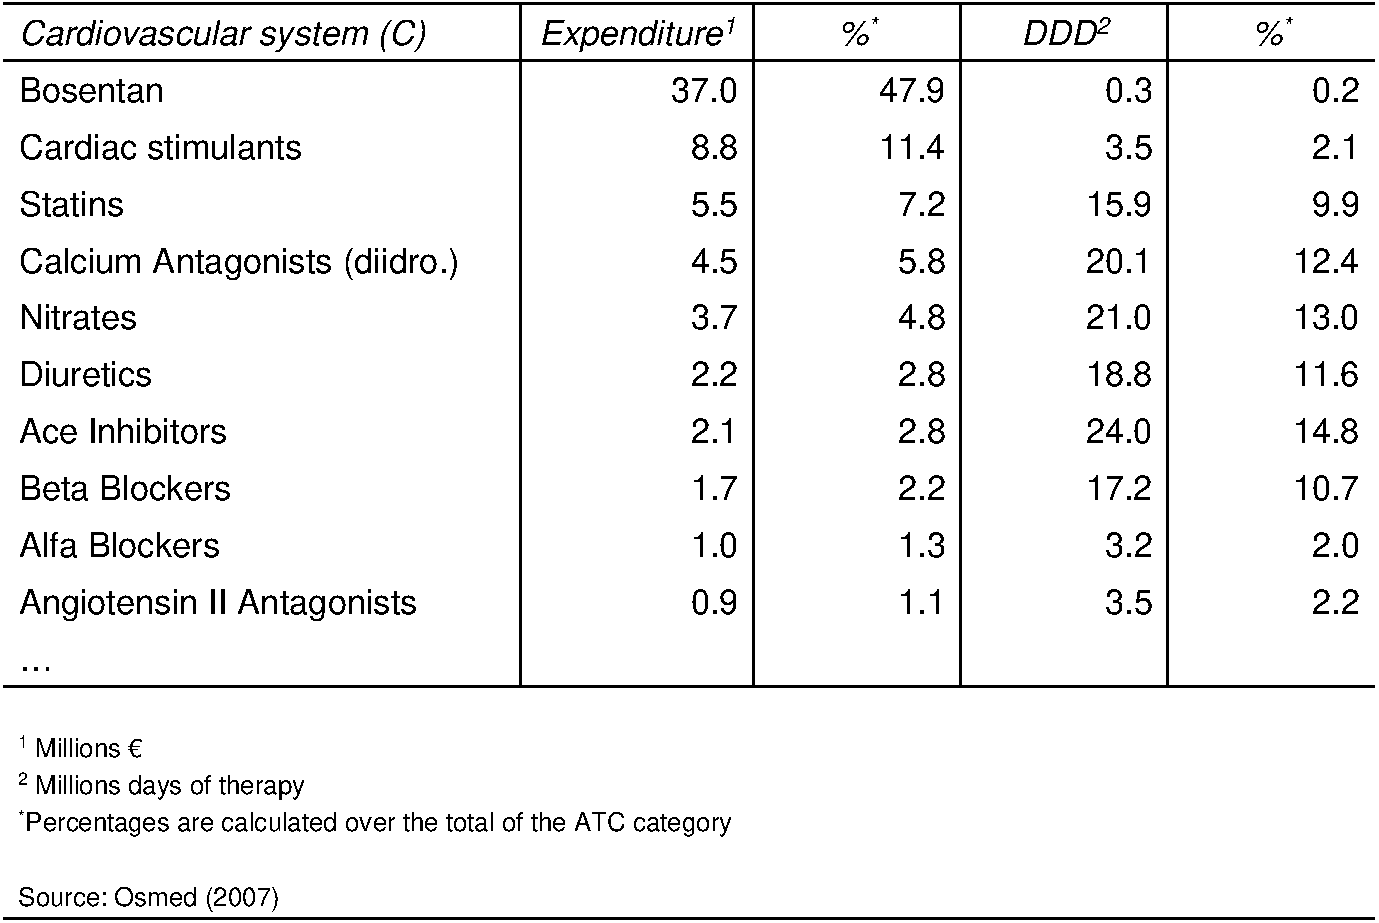
\includegraphics[width=5cm,angle=-90]{/home/gianluca/Dropbox/Unimib/MasterHE/table1}}
%\end{center}
%}

%\frame{%
%\frametitle{}%
%\begin{center}
%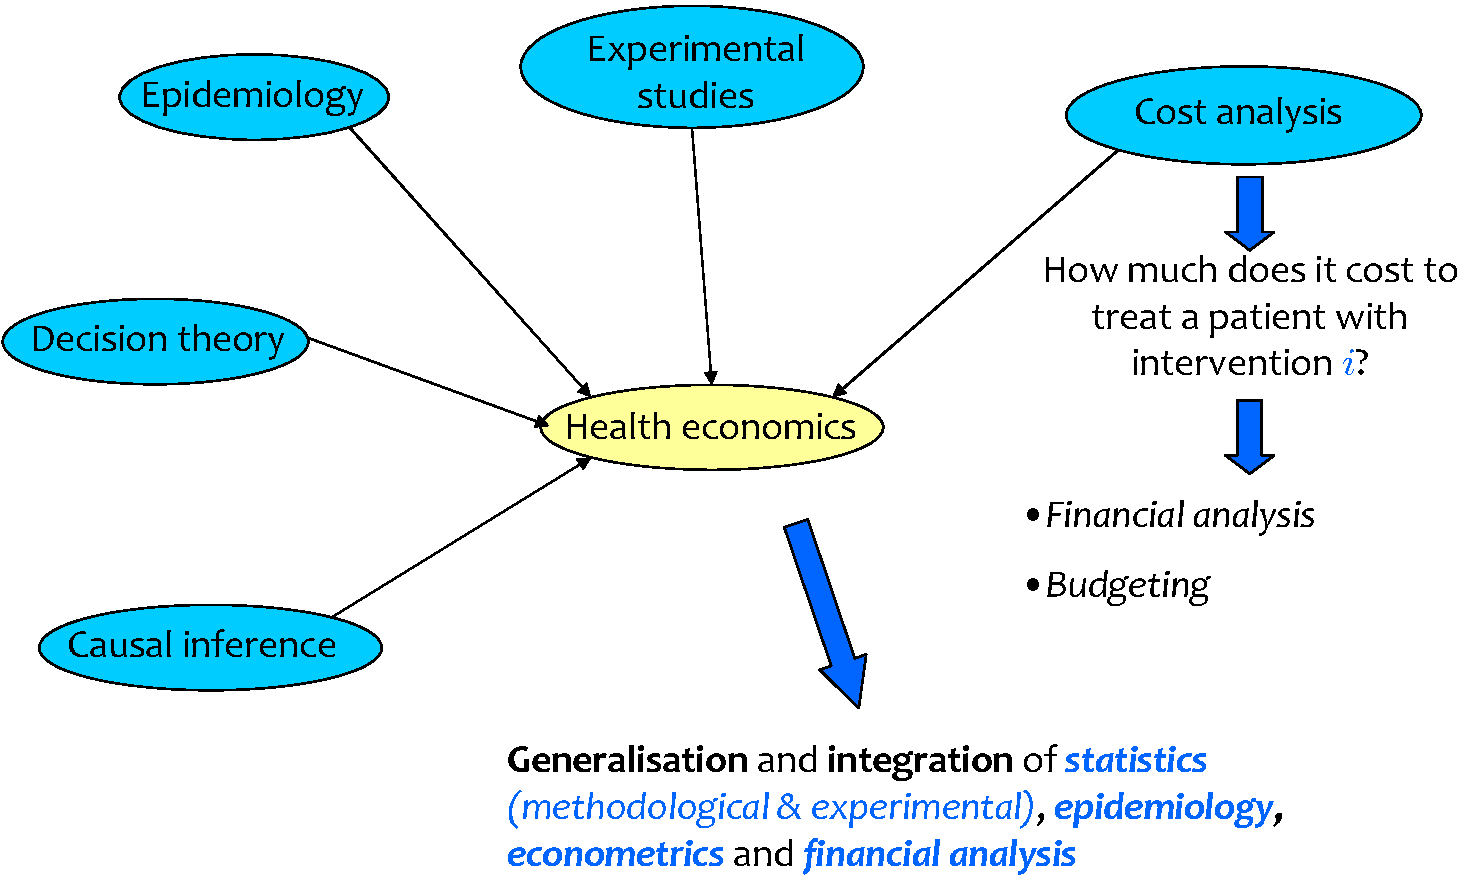
\includegraphics[width=6cm,angle=-90]{/home/gianluca/Dropbox/Unimib/MasterHE/he2New}
%\end{center}
%}


%%%\frame{
%%%\frametitle{}
%%%\vspace{10pt}
%%%\begin{center}
%%%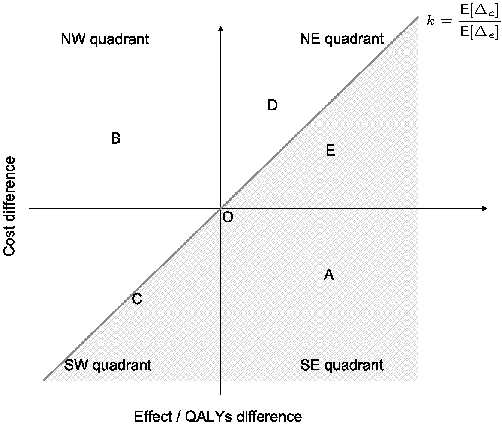
\includegraphics[scale=.4]{/home/gianluca/Dropbox/EcSan/BMHE/Chapters/chapter1/figures/CEPlaneCh1.ps}
%%%\end{center}
%%%\rput(9.4,7.7){\fontsize{7}{8}\selectfont $k=\displaystyle\frac{\mbox{E}[\Delta_c]}{\mbox{E}[\Delta_e]}$}
%%%}

\frame{
\frametitle{}
%%%\begin{center} 
%%%\begin{psmatrix}[rowsep=0.5cm ,colsep=0.9cm]
%%%& & \pscirclebox[linecolor=white,linewidth=.3pt]{\pss{\centering{$\mu_{ct}$}}} & & \pscirclebox[linecolor=white,linewidth=.3pt]{\pss{\centering{$\mu_{et}$}}} \\
%%%
%%%& & & & \pscirclebox[linecolor=white,linewidth=.3pt]{\pss{\centering{$\xi_{t}$}}} &  \pscirclebox[linecolor=white,linewidth=.3pt]{\pss{\centering{$\gamma_{t}$}}} \\
%%%
%%%\pscirclebox[linecolor=white,linewidth=.3pt]{\pss{\centering{$\eta_{t}$}}} & \pscirclebox[linecolor=white,linewidth=.3pt]{\pss{\centering{$\lambda_{t}$}}} & & \pscirclebox[linecolor=white,linewidth=.3pt]{\pss{\centering{$\phi_{it}$}}} & & \pscirclebox[linecolor=white,linewidth=.3pt]{\pss{\centering{$[\tau_{t}]$}}} \\
%%%
%%%& & \pscirclebox[linecolor=white,linewidth=.3pt]{\pss{\centering{$c_{it}$}}} & & \pscirclebox[linecolor=white,linewidth=.3pt]{\pss{\centering{$e_{it}$}}}
%%%
%%%\psset{arrows=->} 
%%%\ncline[linecolor=black,linewidth=.5pt,linestyle=dashed]{1,3}{3,4}
%%%\ncline[linecolor=black,linewidth=.5pt,linestyle=dashed]{2,2}{1,3}
%%%\ncline[linecolor=black,linewidth=.5pt,nodesepA=-3pt,linestyle=dashed]{2,5}{1,5}
%%%\ncline[linecolor=black,linewidth=.5pt,linestyle=dashed]{2,5}{3,4}
%%%\ncline[linecolor=black,linewidth=.5pt]{2,6}{3,4}
%%%\ncline[linecolor=black,linewidth=.5pt]{2,7}{3,4}
%%%\ncline[linecolor=black,linewidth=.5pt,nodesepB=-1pt]{3,1}{4,3}
%%%\ncline[linecolor=black,linewidth=.5pt,nodesepB=-1pt]{3,2}{4,3}
%%%\ncline[linecolor=black,linewidth=.5pt,nodesepB=-1pt,linestyle=dashed]{4,3}{3,4}
%%%\ncline[linecolor=black,linewidth=.5pt]{3,4}{4,5}
%%%\ncline[linecolor=black,linewidth=.5pt]{3,6}{4,5}
%%%\ncline[linecolor=black,linewidth=.5pt,nodesepB=-1pt,linestyle=dashed]{3,1}{1,3}
%%%\ncline[linecolor=black,linewidth=.5pt,nodesepB=-1pt,linestyle=dashed]{3,2}{1,3}
%%%
%%%\end{psmatrix}
%%%\rput(-8.2,-0.5){\psframe[linecolor=red](-1,-0.15)(3.8,4.55)}
%%%\rput(-5.2,-0.5){\psframe[linecolor=blue](-1,0.2)(4.9,4.45)}
%%%\rput(-5.55,4.2){\fontsize{7}{7}\selectfont \red Marginal model for $c$}
%%%\rput(-1.85,4.1){\fontsize{7}{7}\selectfont \blue Conditional model for $e\mid c$}
%%%\end{center}
%%%}

\begin{center} 
\begin{psmatrix}[rowsep=0.01cm ,colsep=.85cm]
& & & \psovalbox[boxsep=false,linecolor=white]{\parbox[l]{1.0cm}{\fontsize{7}{7}\selectfont \sffamily \begin{center}Yes\\ ($p_1$)\end{center}}} & \psovalbox[boxsep=false,linecolor=white]{\parbox[l]{1.8cm}{\fontsize{7}{7}\selectfont \sffamily Cost with NIs + cost influenza}} \\
& \psovalbox[boxsep=false,linecolor=white]{\fontsize{7}{7}\selectfont \sffamily Yes} & \psovalbox[boxsep=false,linecolor=white]{\fontsize{7}{7}\selectfont \sffamily Influenza?} \\
& & & \psovalbox[boxsep=false,linecolor=white]{\parbox[c]{1.0cm}{\fontsize{7}{7}\selectfont \sffamily \begin{center}No\\ ($1-p_1$)\end{center}}} & \psovalbox[boxsep=false,linecolor=white]{\parbox[l]{1.8cm}{\fontsize{7}{7}\selectfont \sffamily Cost with NIs}} \\
\psovalbox[boxsep=false,linecolor=white]{\fontsize{7}{7}\selectfont \sffamily Prophylactic NIs?}\\
& & & \psovalbox[boxsep=false,linecolor=white]{\parbox[l]{1.0cm}{\fontsize{7}{7}\selectfont \sffamily \begin{center}Yes\\ ($p_0$)\end{center}}} & \psovalbox[boxsep=false,linecolor=white]{\parbox[l]{1.8cm}{\fontsize{7}{7}\selectfont \sffamily Cost influenza}} \\
& \psovalbox[boxsep=false,linecolor=white]{\fontsize{7}{7}\selectfont \sffamily \;No} & \psovalbox[boxsep=false,linecolor=white]{\fontsize{7}{7}\selectfont \sffamily Influenza?} \\
& & &\psovalbox[boxsep=false,linecolor=white]{\parbox[c]{1.0cm}{\fontsize{7}{7}\selectfont \sffamily \begin{center}No\\ ($1-p_0$)\end{center}}} & \psovalbox[boxsep=false,linecolor=white]{\parbox[l]{1.9cm}{\fontsize{7}{7}\selectfont \sffamily Cost with no NIs}} \\
\psset{arrows=->} 
\ncangle[angleA=0,angleB=180,ncurv=1,linewidth=.5pt,nodesep=4pt]{4,1}{2,2}
\ncangle[angleA=0,angleB=180,ncurv=1,linewidth=.5pt,nodesep=4pt]{4,1}{6,2}
\ncangle[angleA=0,angleB=180,ncurv=1,linewidth=.5pt,nodesep=4pt]{2,2}{2,3}
\ncangle[angleA=0,angleB=180,ncurv=1,linewidth=.5pt,nodesep=4pt]{6,2}{6,3}
\ncangle[angleA=0,angleB=180,ncurv=1,linewidth=.5pt,nodesep=4pt]{6,3}{7,4}
\ncangle[angleA=0,angleB=180,ncurv=1,linewidth=.5pt,nodesep=4pt]{6,3}{5,4}
\ncangle[angleA=0,angleB=180,ncurv=1,linewidth=.5pt,nodesep=4pt]{2,3}{1,4}
\ncangle[angleA=0,angleB=180,ncurv=1,linewidth=.5pt,nodesep=4pt]{2,3}{3,4}
\ncangle[angleA=0,angleB=180,ncurv=1,linewidth=.5pt,nodesep=4pt]{1,4}{1,5}
\ncangle[angleA=0,angleB=180,ncurv=1,linewidth=.5pt,nodesep=4pt]{3,4}{3,5}
\ncangle[angleA=0,angleB=180,ncurv=1,linewidth=.5pt,nodesep=4pt]{5,4}{5,5}
\ncangle[angleA=0,angleB=180,ncurv=1,linewidth=.5pt,nodesep=4pt]{7,4}{7,5}
\end{psmatrix}
\end{center}
}

\end{document}